% !TEX encoding = cp1250


\chapter{�wiczenie}

\section{�rodowisko - dane o kosa�cach}
Dostarczone dane dotyczy�y wymiar�w dzia�ek kielich�w oraz p�atk�w 150 kosa�c�w z trzech odmian.
Klas� by�a wi�c odmiana kosa�ca przedstawiona w formie liczbowej (0 - kosaciec szczecinkowy, 1 - kosaciec r�nobarwny, 2 - kosaciec wirginijski).
Podczas wszelkich eksperyment�w dane podzielone by�y na zbi�r ucz�cy oraz testowy.

\section{Eksperymenty}
Jedynym parametrem poddanym eksperymentom by�a wielko�� zbioru testowego, zmieniana w zakresie od 1 do 149, co oznacza�o zmian� liczebno�ci zbioru testowego odpowiednio od 149 do 1.

\section{Wyniki}
% TODO

\begin{figure}
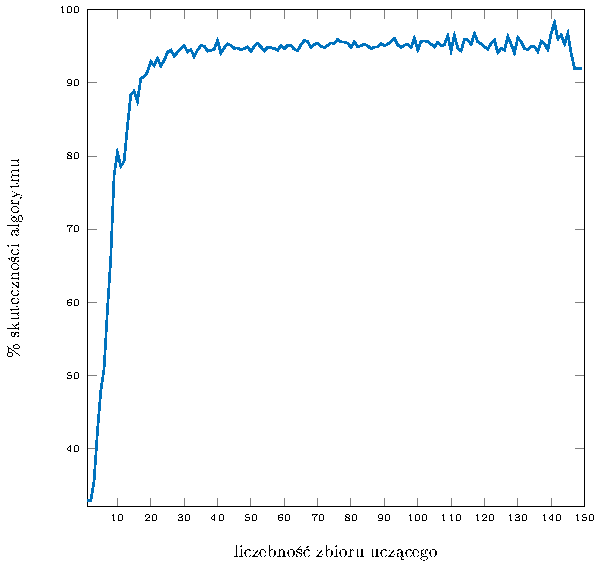
\includegraphics[scale=1]{wykres}
\caption{Wykres przedstawiaj�cy u�rednione wyniki dla wszystkich wielko�ci zbioru ucz�cego}
\label{wyniki}
\end{figure}

\section{Analiza wynik�w}
% TODO


\section{Wnioski}
% TODO